\documentclass{article}
\usepackage[utf8]{inputenc}
\usepackage{amssymb,amsmath}
\usepackage[parfill]{parskip}
\DeclareMathOperator*{\argmin}{arg\,min}
\DeclareMathOperator*{\argmax}{arg\,max}
\usepackage{graphicx}
\usepackage{subcaption}

\usepackage{mathtools}
\DeclareMathOperator{\tr}{tr}

\title{Optimization 10/36-725\\
        Homework 2}
\author{Willie Neiswanger}
\date{}

\begin{document}

\maketitle


\section{Problem Three}

\begin{figure}[h!tbp]
        \center{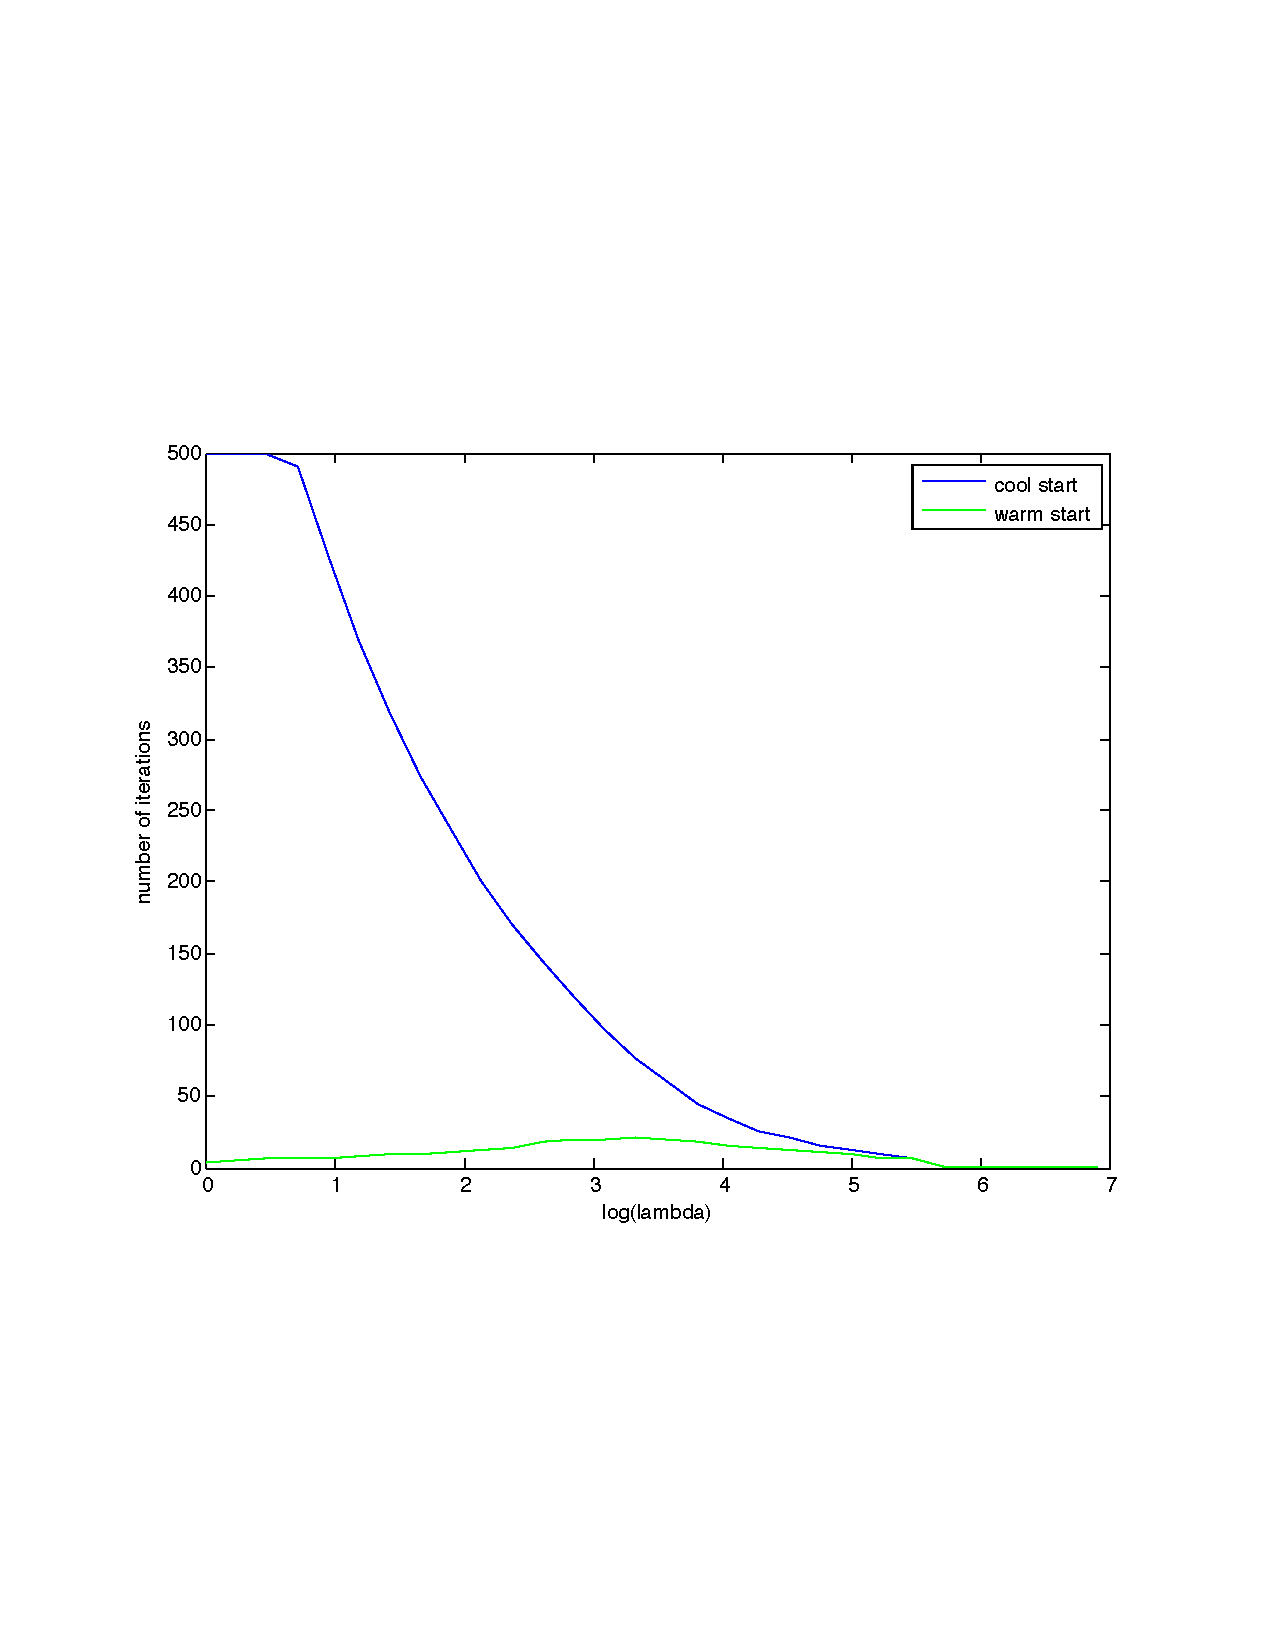
\includegraphics[width=0.7\textwidth]{img/p3_01.pdf}}
       \caption{This plot shows the number of iterations until convergence for both cool and warm
       starts, versus lambda. Warm start yielded better convergence in terms of
       numbers of iterations. Warm starts seem to work because they initialize
       the parameter matrix to a better initial position, and therefore require
       less iterations to arrive at the optimum value.}
\end{figure}

\begin{figure}[h!tbp]
        \center{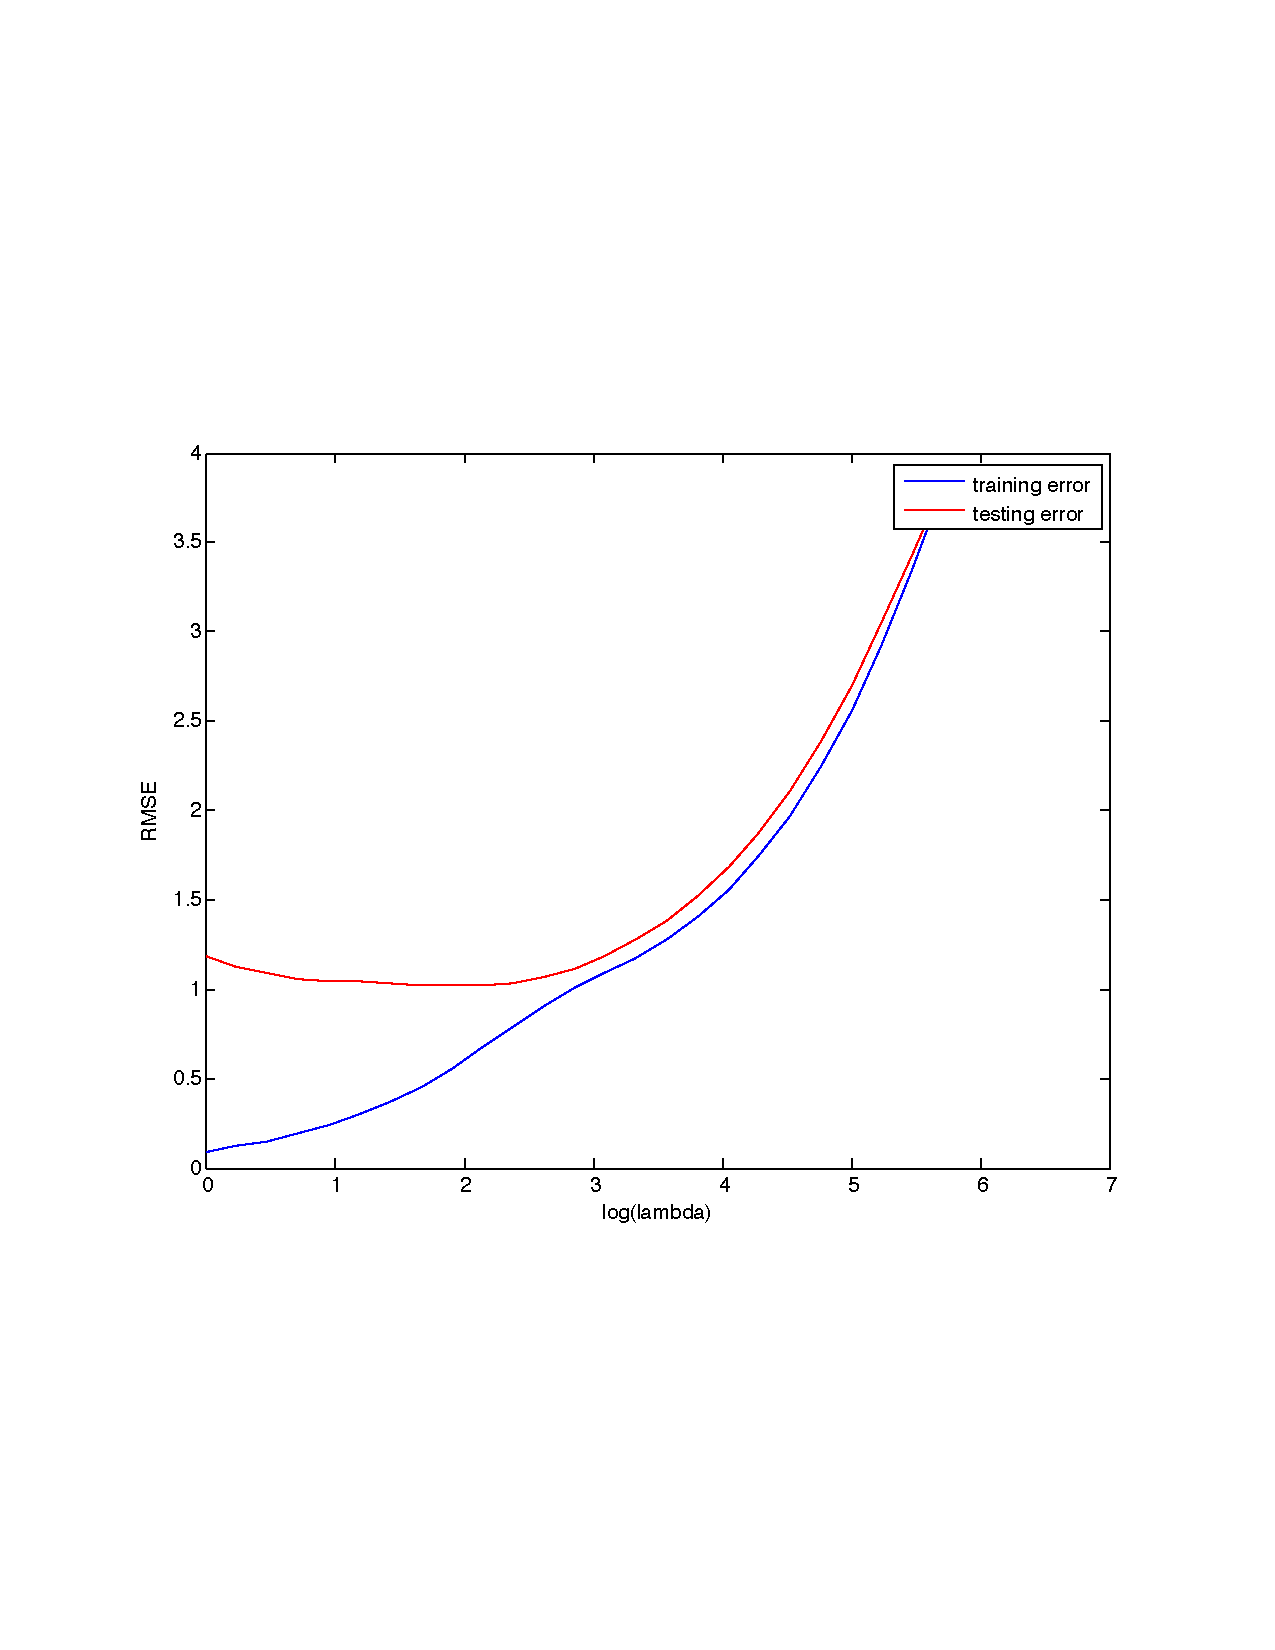
\includegraphics[width=0.7\textwidth]{img/p3_02.pdf}}
        \caption{This plot shows the RMSE of the training and testing error
        versus the log(lambda) value. Based on where the minimum of the test
        error curve occurs, I'd choose lamda = $6.7$ (note this is the true,
        not log(lambda) value).}
\end{figure}

\begin{figure}[h!tbp]
    \centering
    \begin{subfigure}[a]{0.6\textwidth}
        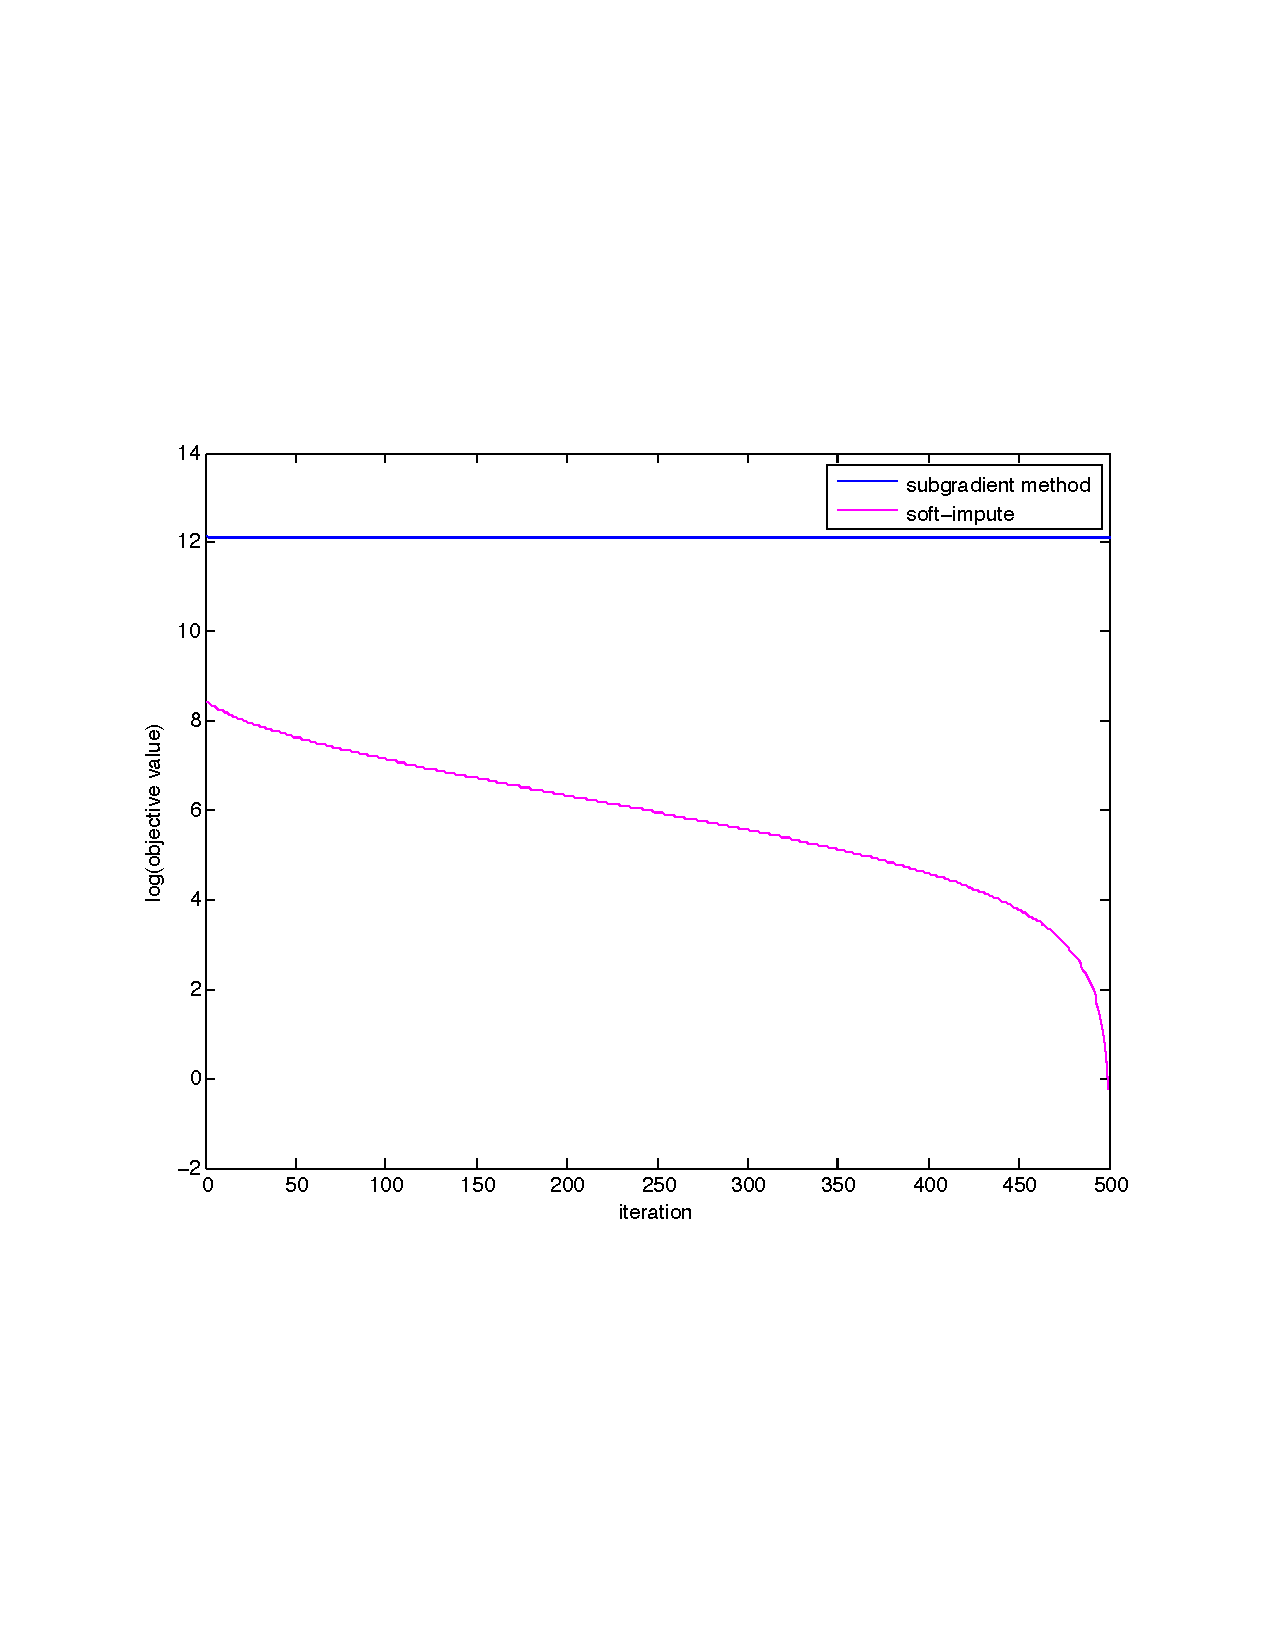
\includegraphics[width=\textwidth]{img/p3_03.pdf}
    \end{subfigure}
    \begin{subfigure}[a]{0.6\textwidth}
        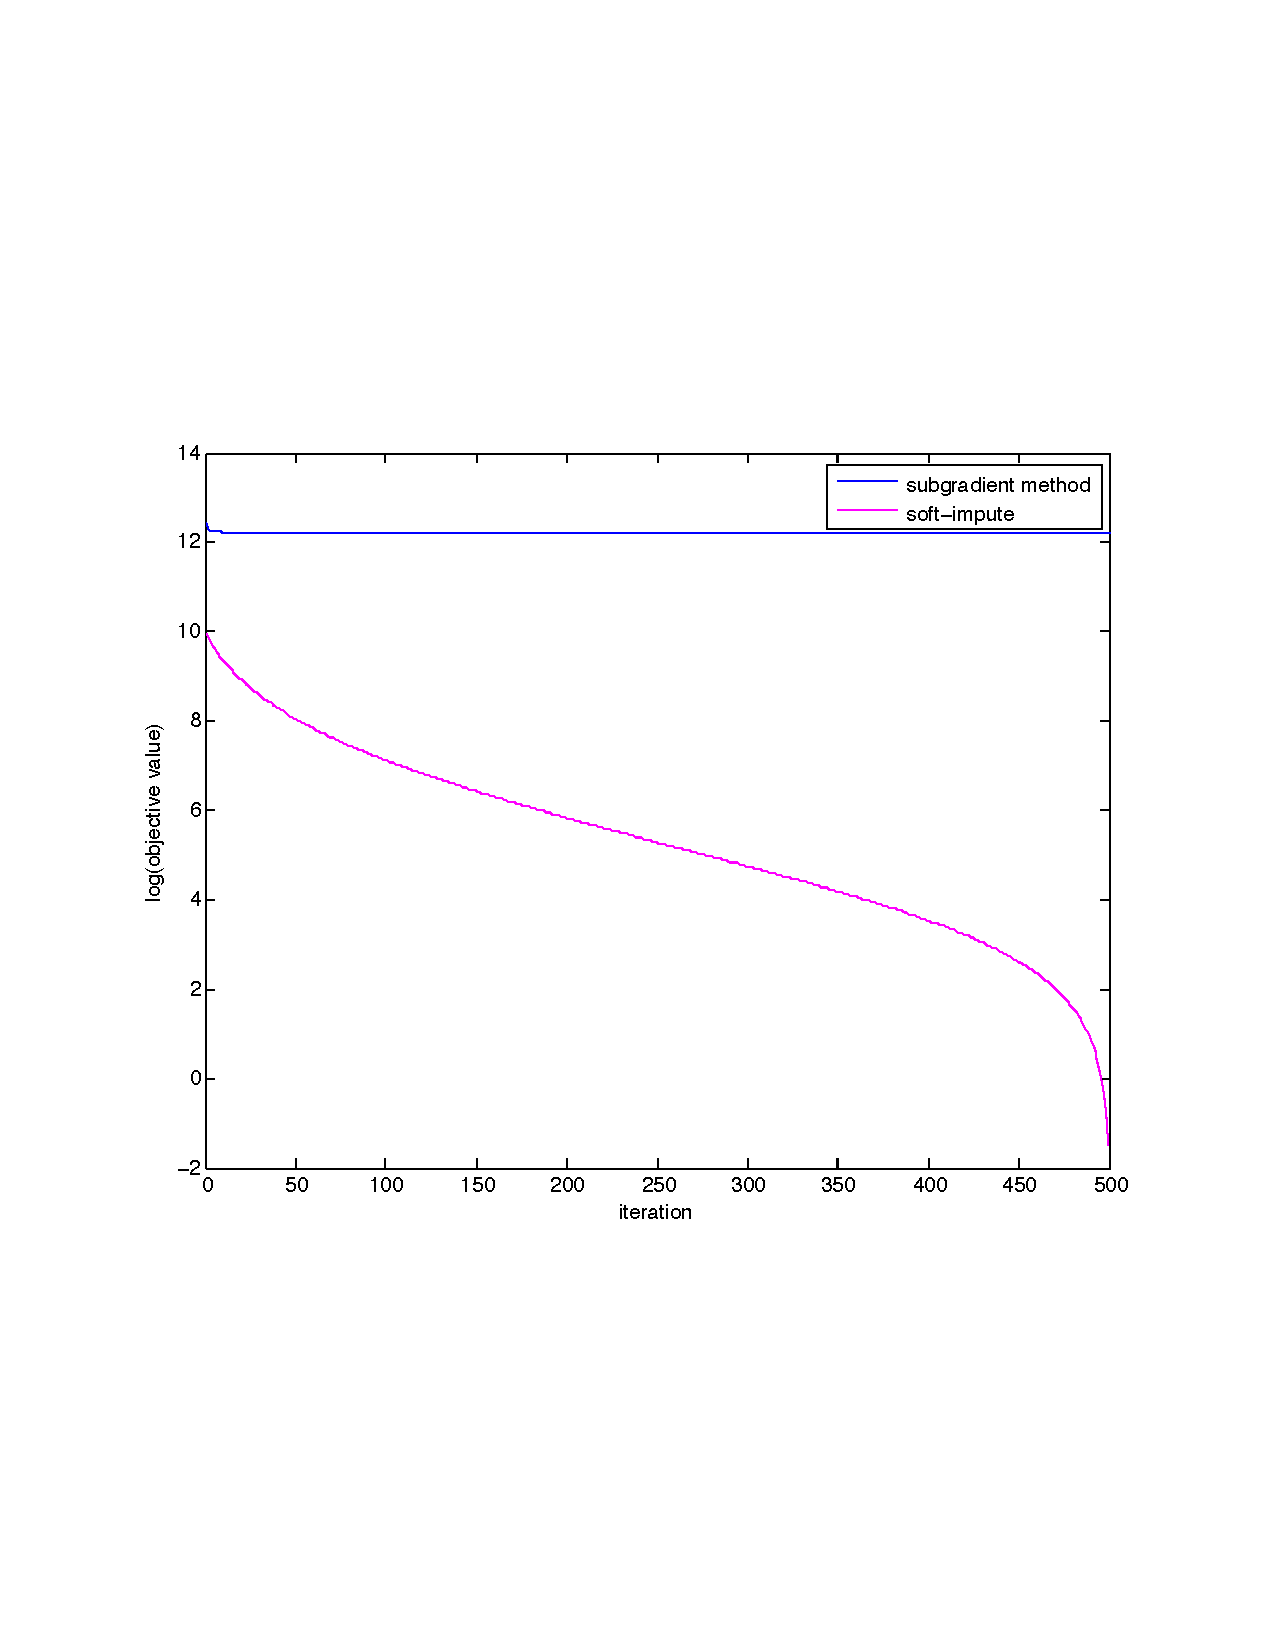
\includegraphics[width=\textwidth]{img/p3_04.pdf}
    \end{subfigure}
    \begin{subfigure}[a]{0.6\textwidth}
        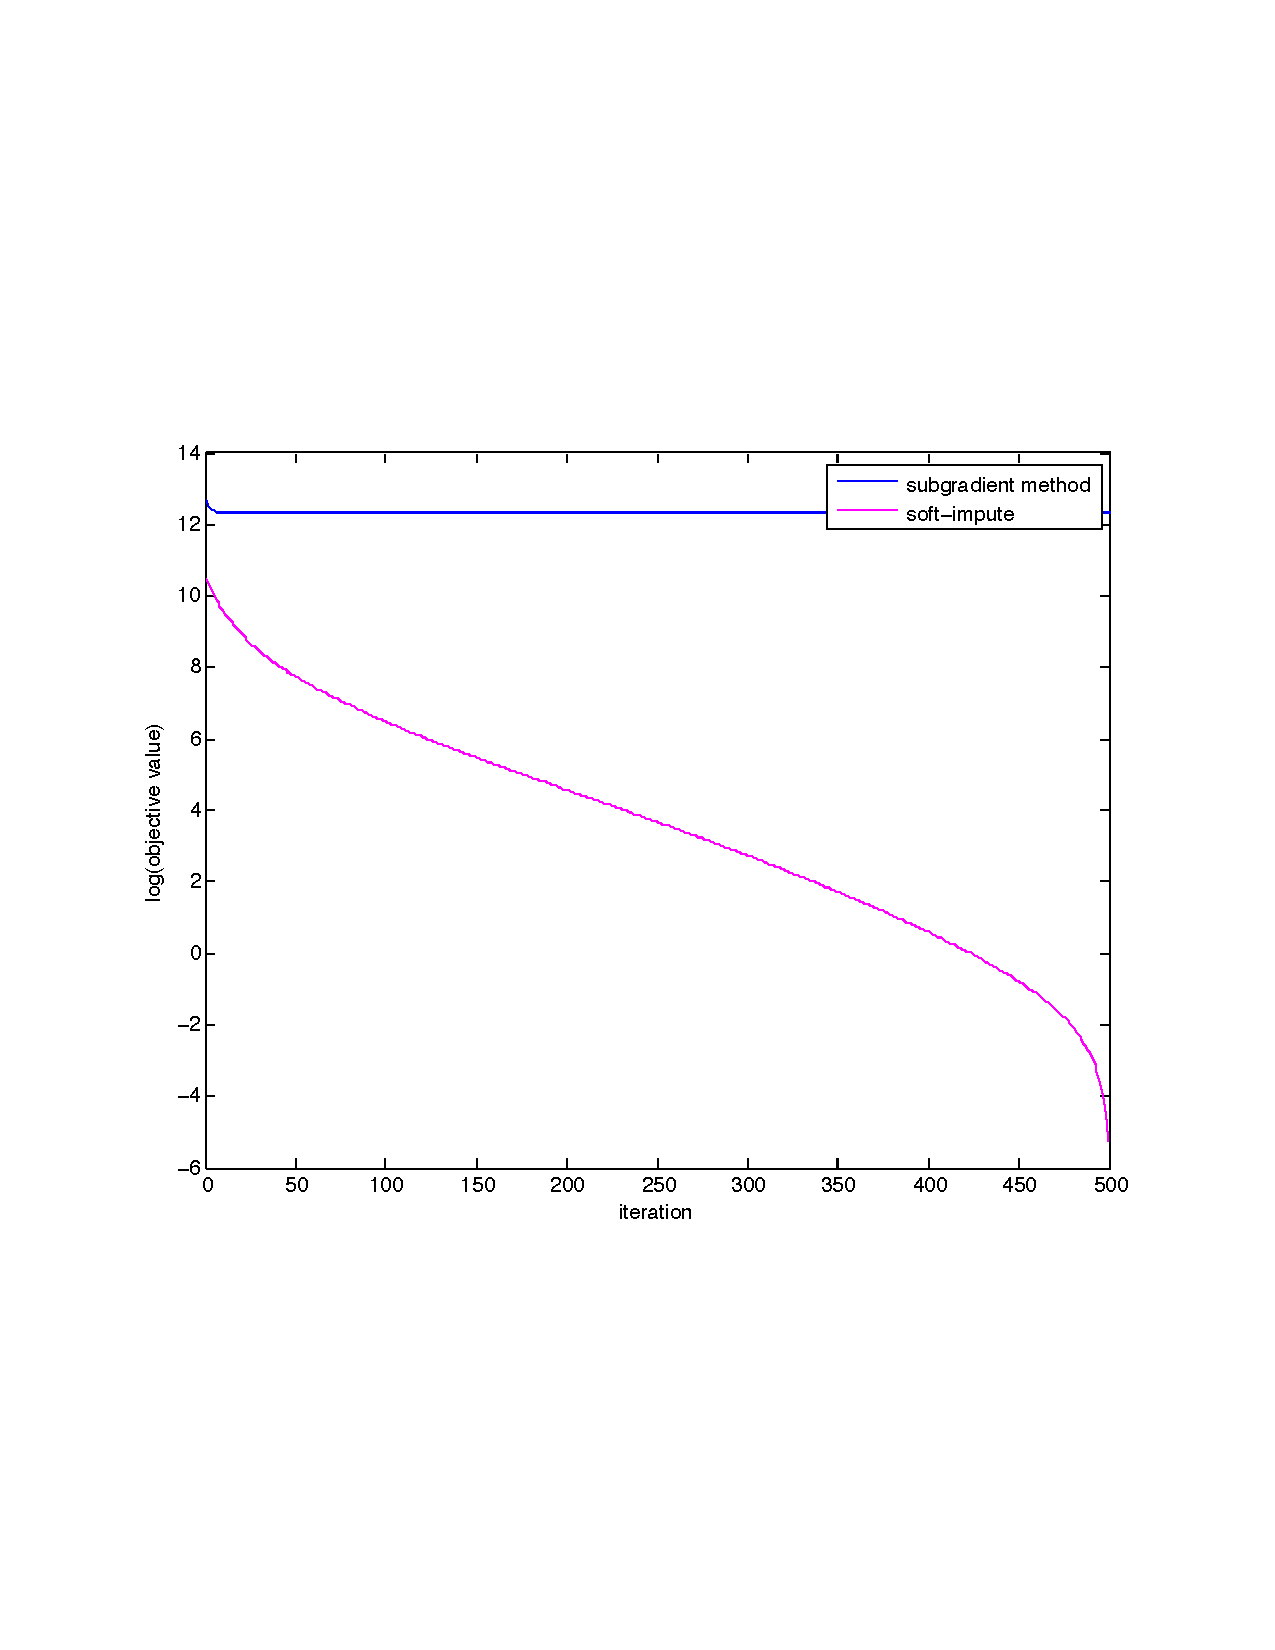
\includegraphics[width=\textwidth]{img/p3_05.pdf}
    \end{subfigure}
    \caption{This plot shows the log(objective-minus-minimum) value vs. iteration, for the
    soft-impute and subgradient methods. Based on this plot, it appears that
    the soft-impute method performed better.} 
\end{figure}

\end{document}
